\documentclass{standalone}
\usepackage{tikz}
\usetikzlibrary{matrix}

\begin{document}
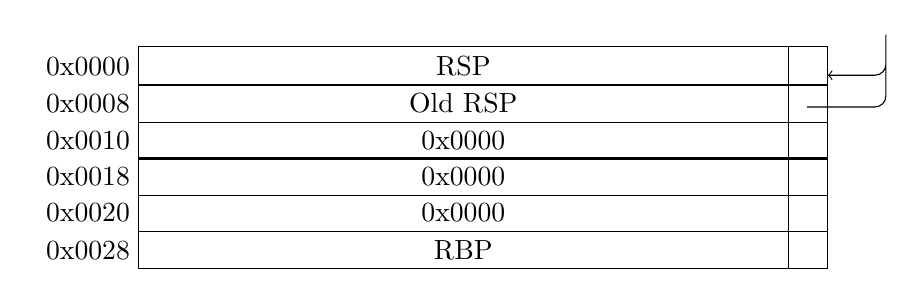
\begin{tikzpicture}

\matrix (m) [matrix of nodes, nodes in empty cells,
column sep=0, row sep=0,
column 1/.style={},
column 2/.style={nodes={text width=8cm,align=center}},
column 3/.style={nodes={minimum width=5mm}}] {
0x0000	&RSP &\\
0x0008	&Old RSP&\\
0x0010	&0x0000&\\
0x0018  	&0x0000  &\\	
0x0020 	&0x0000&\\
0x0028	&RBP   &\\
};

\draw (m-1-2.north west) rectangle (m-6-2.south east);
\draw (m-1-2.north east) rectangle (m-6-3.south east);
\draw (m-4-2.north west) rectangle (m-6-2.south east);
\draw (m-4-2.north east) rectangle (m-6-3.south east);

\foreach \x in {1, 2, 3, 4, 5} {
\draw (m-\x-2.south west) -- (m-\x-3.south east);
};

\draw[->, rounded corners] (m-2-3.mid) -| ++(1cm, 1cm) |- (m-1-3.east);

\end{tikzpicture}
\end{document}